\section{Grundlagen}
\label{sec:grundlagen}

\subsection{Threads}
\label{subsec:threads}
Ein Thread ist ein Ausführungsstrang innerhalb eines Prozesses zur Abarbeitung eines Programms.
Jegliche Threads die durch Java-Code erzeugt werden, oder von der JVM intern genutzt werden,
sind in der HotSpot-JVM als \verb|Kernel-Threads| (oder auch \verb|native threads|) implementiert
und bieten Entwicklern verhältnismäßig leichten Zugriff auf parallelle Programmierung und Synchronisation von Threads.
\parencite[Absatz Thread Management]{OpenJDKHotspotOverview}

\subsubsection{Kernel-Threads}
\label{subsubsec:kernel-threads}
Als \verb|Kernel-Threads| werden Threads bezeichnet dessen Ablaufplanung vom Betriebssystem übernommen wird.
Konkret bedeutet das, das die Zuweisung der Rechenzeit für einen Thread, sowie die Threadwechsel (siehe \ref{subsubsec:threadwechsel})
vom Scheduler \& Dispatcher des Kernels übernommen werden.

Mindestens ein \verb|Kernel-Thread| existiert innerhalb jedes Prozesses, der \verb|Main-Thread|. Kernel-Threads innerhalb eines Prozesses
teilen sich Speicheradressräume, Datei-Handles und Netzwerkverbindungen. Dadurch ist eine Kommunikation zwischen \verb|Kernel-Threads| deutlich
einfacher als bei Prozessen, da Sie über gemeinsamen Speicher verfügen. Allerdings muss eine eventuelle Synchronisation der Threads erfolgen, um
gleichzeitige Zugriffe auf diesselbe Ressource zu verhindern (Deadlock).
Da Sie zudem nur über wenige Ressourcen verfügen (Stack, Registerinhalte, Befehlszähler) ist es, im Vergleich zu Prozessen,
verhältnismäßig günstig Sie zu erstellen oder zu zerstören. \parencite[Kapitel 2.2.5 - Implementing Threads in the Kernel]{Tanenbaum2016}\parencite{Brosenne2021}

\subsubsection{User-Threads}
\label{subsubsec:user-threads}
Die Funktionalität von \verb|User-Threads| \footnote{Auch als Fiber oder virtueller Thread bezeichnet} ist, im Gegensatz zu \verb|Kernel-Threads|
nicht im Kernel implementiert, sondern in einer Programmbibliothek im Benutzeradressraum des Betriebssystems.
Da sich das Scheduling-System des Kernels daher nicht um die Verwaltung dieser Threads kümmern kann muss dies über einen eigenen Scheduling-Algorithmus
der jeweiligen Anwendung erfolgen.
Ein Vorteil dieser Vorgehensweise ist die Möglichkeit, die Schedulingstrategie individuell an die Arbeitslast des Programms anzupassen.

Im Gegensatz zu \verb|Kernel-Threads| kann einem User-Thread, der einen blockierenden Systemaufruf macht, aber nicht vom Scheduler die Kontrolle über die CPU
entzogen werden, da der gesamte Prozess vom Kernel blockiert wird. Aus der Sicht des Kernels existiert lediglich der Main-Thread des Prozesses und dieser
führt einen blockierenden Aufruf aus. \footnote{Hier könne lediglich, abhängig von der Schedulingstrategie des Kernels, ein Prozesswechsel stattfinden}
Daher kann während dieser Zeit kein anderer \verb|User-Thread| des Prozesses ausgeführt werden.

Eine Lösung für dieses Problem ist die Nutzung einer internen, nichtblockierenden API für I/O-Operationen. Dadurch wird lediglich der
auszuführende \verb|User-Thread| blockiert, statt des gesamten Prozesses, und ein weiterer \verb|User-Thread| kann in der Zwischenzeit ausgeführt werden.
\parencite[Kapitel 2.2.4 Implementing Threads in User Space]{Tanenbaum2016}
Diese Vorgehensweise ist im weiteren Rahmen dieser Arbeit von besonderem Interesse und wird in \ref{subsec:nonblocking-i/o} thematisiert.

\subsubsection{Threadwechsel}
\label{subsubsec:threadwechsel}
Sobald die Schedulingstrategie eines Schedulers erfordert, dass ein gerade rechnender Thread die Kontrolle eines logischen CPU an
einen anderen Thread abgeben muss, wird von einem \verb|Kontextwechsel| in Form eines \verb|Threadwechsel| gesprochen.
Ein Threadwechsel kann durch eine Reihe von Ereignissen ausgelöst werden:
\begin{enumerate}
    \item Terminierung eines Threads
    \item Warten auf das Ergebnis einer synchronen I/O-Operation
    \item Verbrauch der zugewiesenen Rechenzeit (Zeitscheibe)
    \item Geringere Priorisierung
    \item Freiwillige Abgabe der CPU-Kontrolle (kooperativ)
\end{enumerate}

Insbesondere das 2. Ereignis ist im Rahmen dieser Arbeit von besonderem Interesse und wird in \ref{subsec:blocking-i/o} thematisiert.

Während bei einem Kontextwechsel von Prozessen (Prozesswechsel) der gesamte Programmkontext (Adressräume, Inhalt der CPU-Register,
Seitentabelle, geöffnete Dateien und Metainformationen)
gewechselt werden muss, wird bei einem Threadwechsel lediglich der Inhalt der CPU-Register (inkl. Programmzähler und Stack-Pointer)
ersetzt.\parencite{Mosberger2002}

\noindent
Da der Threadwechsel, im Fall von \verb|Kernel-Threads|, durch Systemaufrufe, also vom Kernel des Betriebssystems, ausgeführt werden muss, entsteht
bei einem Threadwechsel dennoch ein messbarer Zeitverlust.
Dies ist durch die geringe Geschwindigkeit und den Overhead des notwendigen, vom Dispatcher ausgelösten, Softwareinterrupts bedingt.
Der Softwareinterrupt erfolgt, um die Programmausführung im Benutzer-Modus zu unterbrechen und die Ausführung der jeweiligen Interrupt Service Routine (ISR) im
Kernel-Modus (Kontextwechsel auf privilegierten Ring 0) zu erzwingen, sowie auf dessen Beendigung zu warten.

Bei \verb|User-Threads| sind Threadwechsel extrem effizient und deutlich schneller als bei \verb|Kernel-Threads|
da sie sich komplett im Benutzeradressraum befinden und keinerlei Interaktion mit dem Kernel erfolgt.
Der Prozess führt eine Thread-Tabelle mit, in der der gesamte Thread-Kontext gespeichert ist.
Bei einem Threadwechsel wird der gesamte Thread-Kontext des aktiven \verb|User-Threads| in diese Tabelle gespeichert, und anschließend für den neuen Thread
aus dieser Tabelle in die Maschinen-Register geladen.
\parencite[Kapitel 2.2.6 Thread Scheduling]{Tanenbaum2016}

\subsection{Blocking I/O}
\label{subsec:blocking-i/o}
Bei der herkömmlichen synchronen Ausführung von I/O-Operationen blockiert der entsprechende Funktionsaufruf die Ausführung des
Threads bis die Operation abgeschlossen ist. Das Abschließen der Operation kann zwischen wenigen Millisekunden (Zugriff auf die Festplatte),
einigen Sekunden (Abrufen eines Service oder komplexen Queries) oder länger (bei Benutzer-Interaktion) dauern.
Sobald ein Thread blockiert wird, wird er vom Kernel des Betriebssystems in den Sleep bzw. Waiting-Zustand versetzt.
Wie bereits in \ref{subsubsec:threadwechsel} erwähnt, erfolgt ein Threadwechsel sobald der momentane Thread in einen solchen Zustand
versetzt wird.
Diese Art des Aufrufes von I/O-Operationen wird daher als \verb|Blocking I/O| bezeichnet.
Aus diesem Umstand wird schnell ersichtlich, dass ein auf \verb|Blocking I/O| basierender Webserver nicht in der Lage ist
performant mehrere Anfragen in einem Thread zu bearbeiten, denn sobald der Thread blockiert, werden alle weiteren zu bearbeitenden Anfragen
auch blockiert.
\subsubsection{Thread per Request}
\label{subsubsec:thread per request}
Daher binden Servlet-Container üblicherweise jede vom Webserver weitergeleitete HTTP-Anfrage an einen
Thread im Servlet-API, welcher die jeweilige Anfrage imperativ abarbeitet
(daher auch als\textit{worker thread} bezeichnet). Sie nutzen das \verb|Thread per Request|-Modell.
Der auszuführende Code ist in diesem Ansatz, wie in Abbildung \ref{fig:blocking_thread_per_request}
 an den jeweiligen Thread gekoppelt, und falls ein Thread durch eine I/O-Operation blockiert werden
  die anderen Threads bzw. die zu bearbeitenden Anfragen davon nicht direkt beeinflusst.
\begin{figure}[ht]
	\centering
	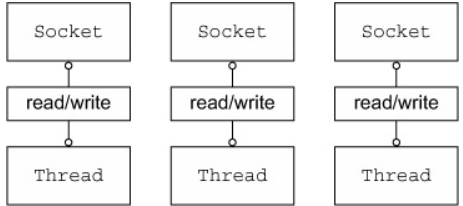
\includegraphics[width=1.0\textwidth]{Blocking-IO-Thread-Per-Request-MultiThread}
	\caption{Thread per Request mit Blocking I/O durch java.nio.channels.selector \parencite{NettyInAction}}
	\label{fig:blocking_thread_per_request}
\end{figure}

Um zu verhindern das für jede Anfrage ein neuer Thread erstellt wird, da dies besonders bei vielen kurzlebigen
 Anfragen einen hohen Overhead erzeugt, und bei einer potentiell hohen Last
unvorhergesehen viele Ressourcen des Betriebssystems verwendet werden, wird das \verb|Thread per Request|-Modell 
in der Regel um einen \verb|Threadpool| erweitert. 
Dabei wird eine begrenzte Anzahl an Threads bereits im vornherein erstellt und wiederverwendet, wodurch sich die Kosten der Threaderstellung
zur Laufzeit amortisieren und die benötigten Ressourcen begrenzt werden.
Anfragen können solange parallel ausgeführt werden bis die Anzahl der gleichzeitigen Anfragen die
Anzahl der Threads im \verb|Threadpool| übersteigt. 
Bei diesem Punkt, müssen eingehende Anfragen solange warten, bis ein Thread wieder verfügbar ist.
Der Grad der Parallelität ist bei diesem Ansatz durch die Größe des Threadpools begrenzt.

\subsection{Nonblocking I/O}
\label{subsec:nonblocking-i/o}
APIs die \verb|Blocking I/O| basieren blocken also den Thread bis die Operation abgeschlossen ist, und verursachen somit
immer einen Threadwechsel. 
Ressourcenzugriffe in \verb|Nonblocking I/O|-APIs kommen hingegen sofort zurück und blockieren der Thread nicht.
Dieser kann dadurch den weiteren Code des Programms ausführen. 
Sobald das Ergebnis des Zugriffs bereit ist, wird der Aufrufer darüber informiert.

Die Grundlage für diese Funktionsweise wird durch einen Mechanismus namens \verb|Synchronous Event Demultiplexing|
 bzw. \verb|Event notification API| durch jedes moderne Betriebssystem bereitgestellt.

\subsubsection{Synchronous Event Demultiplexing}
\label{subsubsec:event demultiplexing}
Der Begriff Demultiplexing beschreibt dabei das Aufteilen eines, aus mehreren Signalen zusammengesetzes, Signals 
in seine ursprünglichen Komponenten.

Mit diesem Mechanismus lässt sich eine Menge an Ressourcen (bspw. Sockets oder Dateihandles) beobachten. 
Sobald eine I/O-Operation, die auf einer der Ressourcen ausgeführt wurde, abgeschlossen ist, gibt der Demultiplexer eine Menge an Events
zurück, die die Daten enthalten und Auskunft über den Zustand der Ressource geben.

\verb|Synchronous Event Demultiplexing| bzw. die \verb|Event notification API| wird in Linux durch \verb|epoll|, in BSD mit \verb|kqueue| und in 
Windows durch \verb|IOCP| bereitgestellt.\footnote{Auf alten Systemen wird als Fallback die POSIX Funktion \textit{select()} genutzt.}

2002 wurde Unterstützung für nichtblockierende I/O-Operationen in Java mit dem \verb|java.nio|-Paket eingeführt.
Dies basiert auf den genannten Betriebssystem-Schnittstellen und abstrahiert diese.\parencite{OpenJDKNIO} 
Dabei ist \verb|java.nio.channels.selector| der Dreh- und Angelpunkt und gibt Auskunft darüber, welche 
beobachteten Ressourcen bereit für I/O-Operationen sind. 

Abbildung \ref{fig:nonblocking_single_thread} stellt dar, wie mehrere Ressourcen über die 
\verb|java.nio|-APIs überwacht werden können.


\begin{figure}[ht]
	\centering
	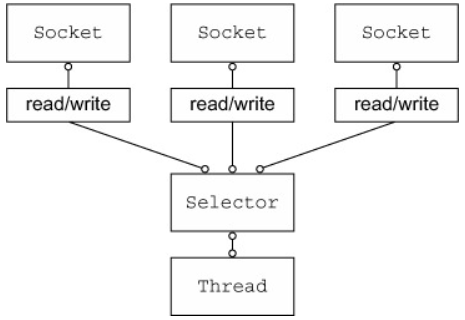
\includegraphics[width=0.8\textwidth]{Nonblocking-IO-EventNotificationAPI-SingleThread}
	\caption{Nonblocking I/O durch java.nio.channels.selector \parencite{NettyInAction}}
	\label{fig:nonblocking_single_thread}
\end{figure}


Im Gegensatz zum beschriebenen \verb|Thread per Request|-Modell, können durch \verb|Nonblocking I/O|
mehrere Anfragen parallel von einem Thread verarbeitet werden. Daher die Bezeichnung \verb|Single Threaded| Modell. 
Dies resultiert in einer geringenen Anzahl an benötigten Threads und demnach auch in weniger Threadwechseln.
Darüber hinaus wird die Möglichkeit eines gleichzeitigen Ressourcenzugriffs von mehreren Threads eines Prozesses
durch die Nutzung eines einzigen Threads unterbunden und eine Thread-Synchronisation ist nicht erforderlich.

Der Aufruf des \verb|Synchronous Event Demultiplexers| selber ist blockierend (daher auch der Zusatz \verb|Synchronous|)
 und zwar solange bis mind. eine Ressource ein bereit für eine I/O-Operation ist 
 \footnote{Ein typischer Polling-Algorithmus würde, durch die geringe Verfügbarkeit der Ressourcen, 
 viel CPU-Rechenzeit verschwenden}. 
 Sobald dies passiert ist der Aufruf beendet und eine Menge an Events wird an den Aufrufer zurückgegeben.

\subsubsection{Event Loops}
\label{subsubsec:event loops}
Ein beliebtes Modell für die Verarbeitung von asynchronen Events ist die \textit{Event Loop}.
Sobald ein Event entsteht wird es einer Warteschlange (Queue) in der Event Loop hinzugefügt.
Solange der ausführende Thread aktiv ist und die Queue Events enthält, wird in einer Schleife das nächste Event
abgerufen und vollständig verarbeitet bevor die nächste Iteration beginnt.

\begin{figure}[ht]
	\centering
	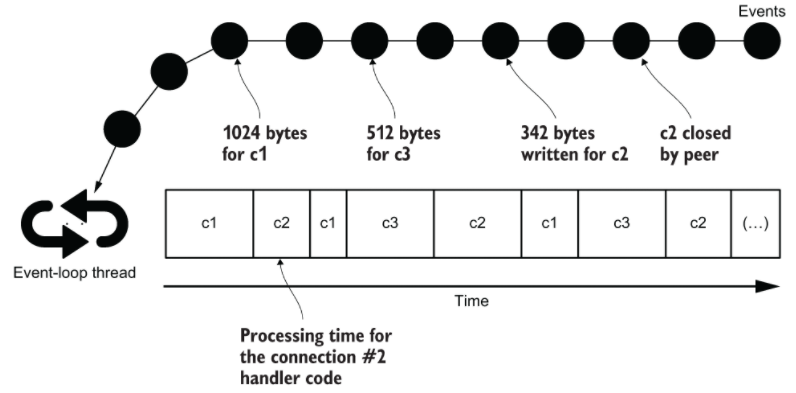
\includegraphics[width=1.0\textwidth]{EventLoop}
	\caption{Exemplarische Abbildung einer Event Loop. \parencite[Kapitel 1.7]{Ponge2020}}
\end{figure}

Dies können beispielsweise I/O-Events sein, die signalisieren das Daten bereit zur Weiterverarbeitung sind, aber auch jegliches andere Event.
Eine Event Loop wird in der Regel auf einem einzigen Thread, dem \verb|IO-Thread| oder \verb|Event-Loop Thread|
 ausgeführt, daher darf das Verarbeiten von Events keine blockierenden, oder zeitintensiven Operationen beinhalten.

Dieses Modell wurde zuerst vorrangig in den JavaScript-Engines von Webbrowsern als Nebenläufigskeitsmodell genutzt,
 da JavaScript kein Multithreading
unterstützt,\parencite{MozillaEventLoop} und später auch von der Node.js-Laufzeitumgebung,
um jegliche I/O-Operationen auf nicht-blockierende Art in einem einzigen Thread auszuführen.\parencite{NodeJSEventLoop}

Für ein laufendes Programm muss der, in \ref{subsubsec:event demultiplexing} beschriebene 
\verb|Synchronous Event Demultiplexing|-Mechanismus natürlich mehrmals aufgerufen werden.

Ein veranschaulichendes Pseudocode-Beispiel, wie ein Synchronous Event Demultiplexer während der 
gesamte Programmlaufzeit aktiv ist und dessen zurückgegebene Events verarbeitet werden,
wird in Listing \ref{lst:EventLoop_Pseudocode} dargestellt.
\begin{lstlisting}[caption=Einfaches Pseudocode-Beispiel für Synchronous Event Demultiplexing mit Event Loop),
	 captionpos=b, label=lst:EventLoop_Pseudocode]
	 //add resources to a data structure and associate them with a specific operation
	 watchedList.add(socketA, FOR_READ)                            
	 watchedList.add(fileB, FOR_READ)
	 //Note: this call is synchronous and blocks until a resource is ready for an i/o-operation
	 while (events = demultiplexer.watch(watchedList)) {
	   // event loop -  process the returned events from the demultiplexer
	   for (event of events) {
		 // This read will never block and will always return data
		 // The resource is guaranteed to be ready for read
		 data = event.resource.read()
		 if (data == RESOURCE_CLOSED) {
		   // the resource was closed, remove it from the watched list
		   demultiplexer.unwatch(event.resource)
		 } else {
		   // some actual data was received, process it - dont block here with a long running operation
		   consumeData(data)
		 }
	   }
	 }
\end{lstlisting}\parencite[Event Demultiplexing]{NodeJSDesignPatterns}

\subsubsection{Reactor-Pattern}
Das \verb|Reactor-Pattern| ist eine spezielle Form der beschriebenen Algorithmen und wurde bereits 1995 beschrieben.\parencite{SchmidtReactorPattern}
Die Hauptidee besteht darin jedem Event einer Ressource einen Event-Handler zuzuordnen. 
Dieser wird aufgerufen sobald das Event entsteht und von der \verb|Event Loop| abgearbeitet wird. 

\begin{figure}[ht]
	\centering
	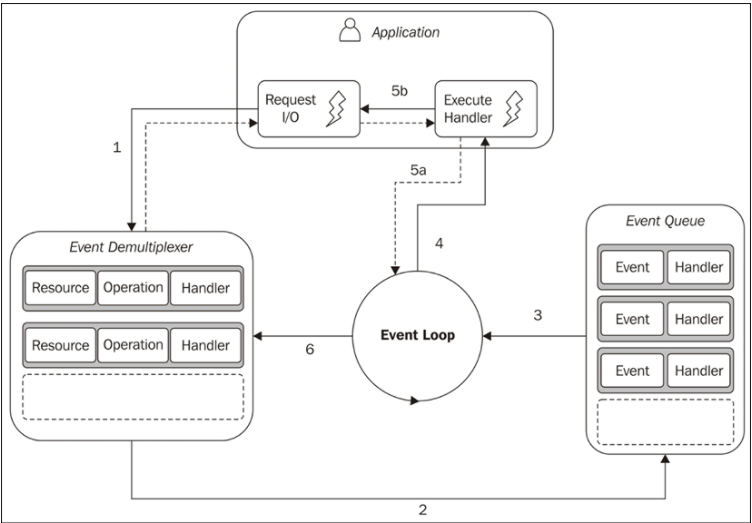
\includegraphics[width=0.8\textwidth]{reactor_pattern}
	\caption{Reactor Pattern \parencite[Abbildung 1.3]{NodeJSDesignPatterns}}
	\label{fig:reactor_pattern}
\end{figure}

Zu Beginn generiert die Anwendung eine neue I/O-Operation indem eine Anfrage an den \verb|Event Demultiplexer| gestellt wird.
Dabei spezifiziert die Anwendung zudem einen Handler, welcher aufgerufen wird sobald die Operation abgeschlossen wurde.
Das Verschicken einer Anfrage an den Event Demultiplexer ist ein nicht-blockierender Aufruf und gibt sofort die Kontrolle
an die Anwendung zurück.
Sobald eine Menge von I/O-Operationen abgeschlossen ist, schiebt der Event Demultiplexer eine Menge an entsprechenden Events 
in die \verb|Event Queue|.
Die \verb|Event Loop| iteriert über die Element der \verb|Event Queue| und ruft für jedes Event den dazugehörigen Handler auf.
Der Event-Handler, der Teil des Anwendungscodes ist, gibt die Kontrolle an die \verb|Event Loop| zurück, sobald seine Ausführung
beendet ist. 

Wärend der Event-Handler ausgeführt wird, kann er neue asynchrone Operationen ausführen, durch die wiedderum 
neue Elemente bzw. Ressourcen zum \verb|Event Demultiplexer| hinzugefügt werden.
Sobald alle Elemente in der \verb|Event Queue| verarbeitet wurden, blockiert die \verb|Event Loop| solange 
bis vom \verb|Event Demultiplexer| neue Events der \verb|Event Queue| hinzugefügt werden. \parencite{SchmidtReactorPattern}

Das Reactor-Pattern wird unter Anderem von der JavaScript-Laufzeitumgebung Node.js und vom Java-Framework \verb|Netty| implementiert.

\paragraph{Netty}
Die \verb|java.nio|-API bietet lediglich die Grundlage für asynchrone Anwendungen 
durch die Schnittstelle für die Nutzung von \verb|Nonblocking I/O|.
Sie gibt aber kein Threading-Modell vor, bietet keine Unterstützung für Protokolle höherer Level (beispielsweise HTTP) und 
kann die asynchronen I/O Events nicht verarbeiten, weswegen Entwickler in der Praxis selten direkt mit der \verb|java.nio|-API
konfrontiert sind.

Diese nicht-trivialen Aufgaben werden, auf der Basis von \verb|java.nio|, durch das Client-Server Framework \verb|Netty| implementiert.
Dabei handelt es sich um ein asynchrones, eventgesteuertes Framework für netzwerkorientierte Anwendungen und simplifiziert 
die Programmierung von Netzwerk-Komponenten, wie TCP- oder UDP-Socket Server. \parencite{NettyUserAction}